\documentclass{article}

\usepackage{Engineering}
\pdftitle{EFPLAB_1}

% === TEXT ===
\title{\textbf{Energies, fluids \& processes -- Laboratory \\ HSLU, Semester 2}}
\author{Matteo Frongillo}
\date{}

\begin{document}

\maketitle
\tableofcontents
\pagebreak

\section{Introduction to energies, fluids, and processes}
Energy exists in different forms and can neither be destroyed nor generated, but only
transformed.

\subsection{Energy forms}
\begin{minipage}{.45\textwidth}
    \begin{itemize}[itemsep=6pt]
        \item Potential energy: $E = mgh$
        \item Kinetic energy: $E = \frac{1}{2}mv^2$
        \item Thermal energy: $E = mc_p\Delta T$
        \item Light energy: $E = h\nu$
    \end{itemize}
\end{minipage}
\hfill
\begin{minipage}{.45\textwidth}
    \begin{itemize}[itemsep=6pt]
        \item Chemical energy: $E = mH$
        \item Electrical energy: $E = k\dfrac{q_1 q_2}{r}$
        \item Nuclear energy: $E = \Delta mc^2$
        \item Pressure energy (acoustic): $E = \dfrac{m p}{\rho}$
    \end{itemize}
\end{minipage}

\section{Fluids as energy carriers}
\subsection{Fluid definition}
\dots

\subsubsection{Properties of a fluid}
\pph{Density $\rho$}
Densitiy is a measure of working potential of a fluid:
\figbox{$\rho \triangleq \dfrac{m}{V}\ \left[\dfrac{kg}{m^3}\right]$}

where:
\begin{itemize}
    \item $m$ = mass;
    \item $V$ = volume.
\end{itemize}

\begin{center}
    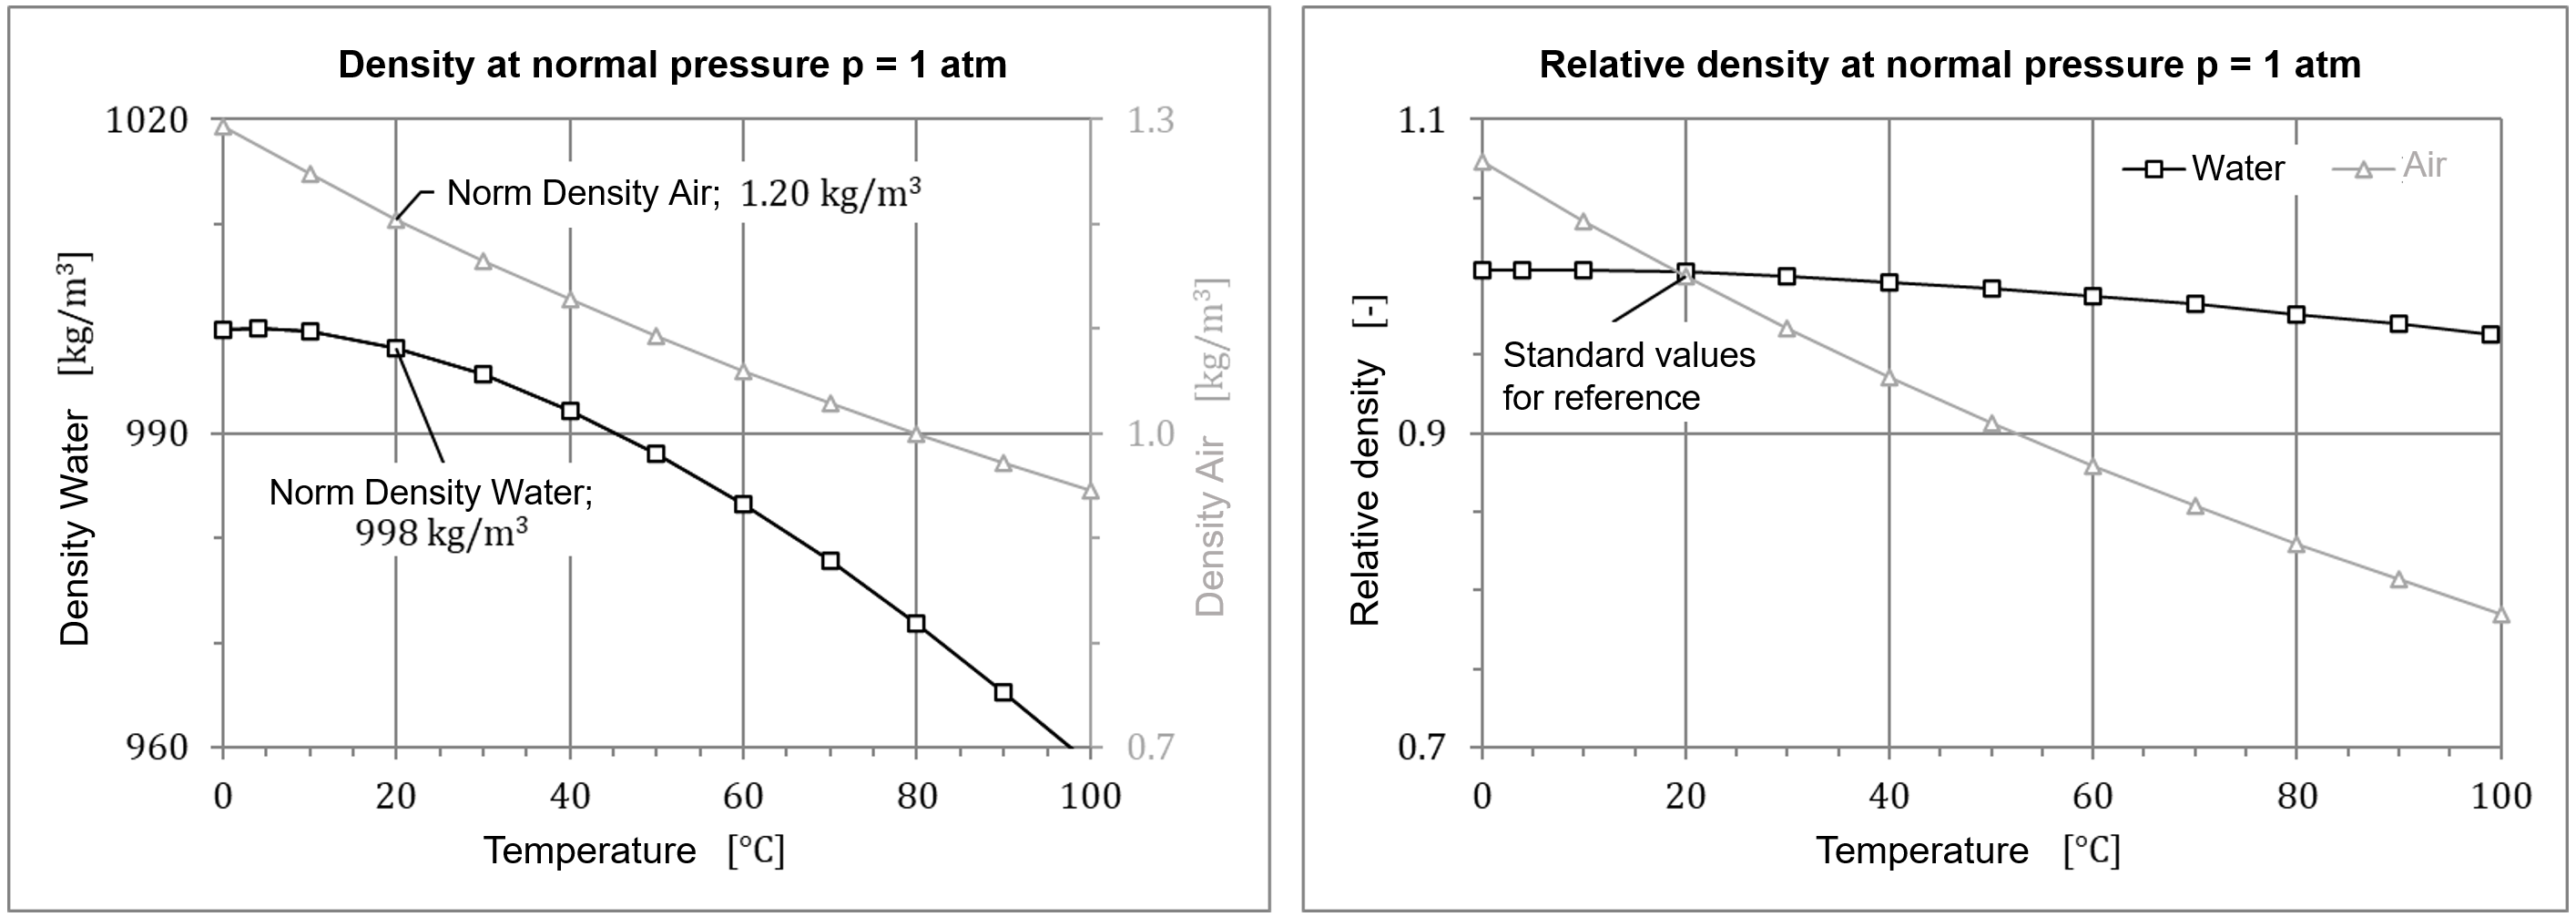
\includegraphics[width=\textwidth]{media/Dichte_rhoT_en.PNG}
    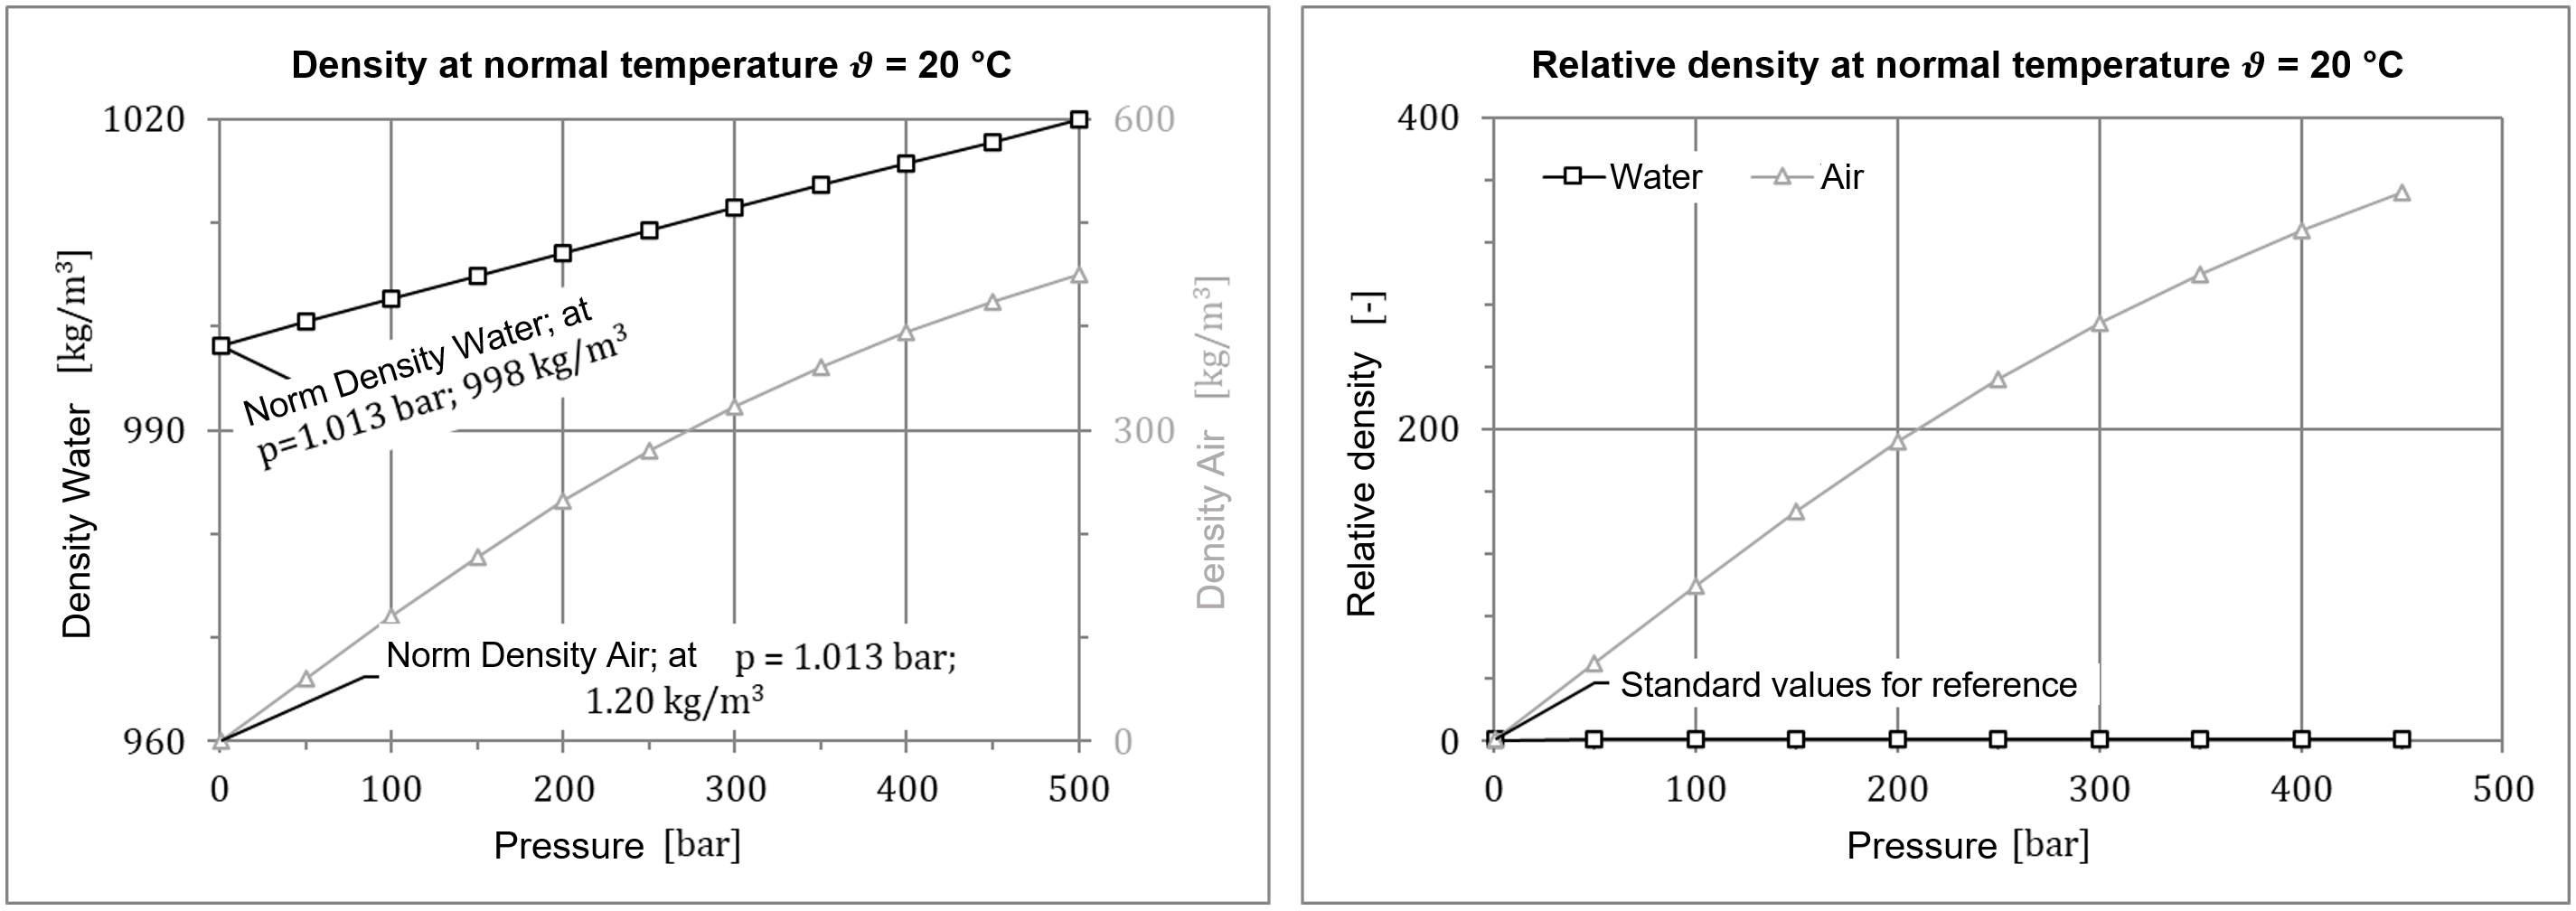
\includegraphics[width=\textwidth]{media/Dichte_rhop_en.png}
\end{center}

\pph{Kinematic viscosity $\nu$}
Viscosity is a measure of the specific loss capacity of a fluid:
\figbox{$\nu \triangleq \dfrac{\mu}{\rho}\ \left[\dfrac{N\cdot s}{m^2} = Pa\cdot s\right]$}

where:
\begin{itemize}
    \item $\mu$ = dynamic viscosity
    \item $\rho$ = density
\end{itemize}

\begin{center}
    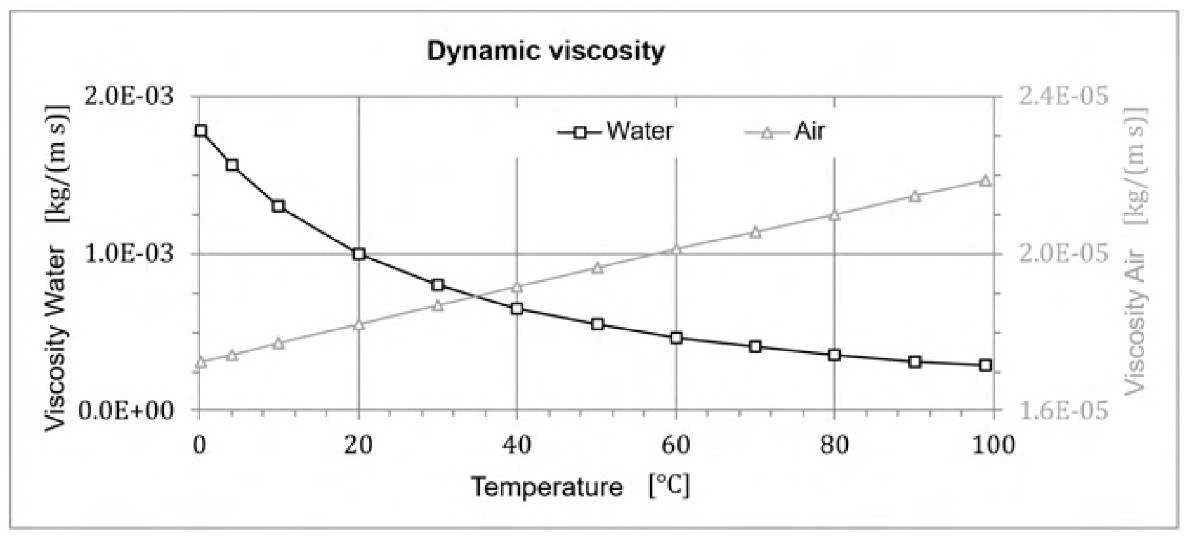
\includegraphics[width=.74\textwidth]{media/viscosity.png}
\end{center}

Viscosity of a liquid fluid \textbf{decreases} with increasing temperature,
while viscosity of a gaseous fluis \textbf{increases} with increasing temperature.

\rem{$\nu \propto \dfrac{1}{T}$}

\pph{Compressibility}
An increase in pressure on a given fluid mass causes compression and thus
lead to a reduction in volume.

Mach number is a non-dimensional number that relates the fluid velocity
to the sound velocity (in air):
\figbox{$M = \dfrac{u}{c}$}

\note{Since Mach number normally is very small, it can be neglected from calculations.}

\subsection{Real and ideal fluids}
\subsubsection{Real fluid}
All fluids are real fluids and have real fluid properties. This means
that they are compressible and exhibit frictional losses during the flow process.
Physically, this means they have a viscosity $\nu > 0$.

\subsubsection{Ideal fluid}
A fluid can be simplified as an ideal fluid assuming a constant density
(incompressible) and a viscosity $\nu = 0$ (frictionless).

\newpage
\subsection{Technical application flows}
\subsubsection{Internal flow (flow through)}
Fluids that flow through a body (pipes, ducts, machines, ...).

Internal losses (such as friction, pressure, and fluid force) are relevant for the calculation of internal flows.

\subsubsection{External flow (flow around)}
Fluids that flow around bodies (motor vehicles, aircraft, buildings, ...).

External losses (such as velocity, pressure, density, and temperature
near and far from bodies) are relevant for the calculation of external flows
and aerodynamics.

\subsection{Forces for fluid motion}
\subsubsection{1D flow in $x$ direction}
\begin{center}
    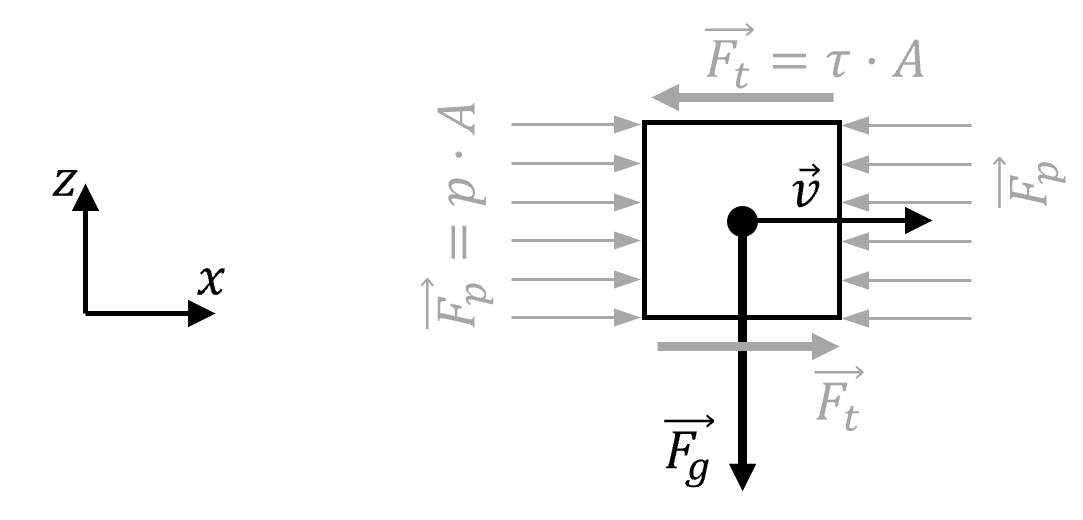
\includegraphics[width=.6\textwidth]{media/Kraftgleichgewicht.png}
\end{center}

Surface forces act on the interfaces of a fluid body and are introduced by
direct contact of the environment. Fluids also cause surface forces on
their surroundings.

\pph{Forces decomposition}
Surface forces:
\begin{itemize}
    \item $F_t = \tau\cdot A$: shear force (tangential to the surface);
    \item $F_p = p\cdot A$: fluid pressure force.
\end{itemize}

Body forces:
\begin{itemize}
    \item $F_g = F\cdot g\cdot \cos\theta$: gravitational force (perpendicular to the surface);
    \item $F_n = -F\cdot g\cdot \cos\theta$: normal force (perpendicular to the surface);
    \item $F_v$: inertial force.
\end{itemize}

Inertial forces will always destabilize the flow field.

Viscous forces will always stabilize the flow field.

\newpage
\subsection{Laminar and turbolent flow}
A flow that flows in an orderly manner is called laminar flow. In contrast,
flows with vortices are called turbolent flow.

\begin{center}
    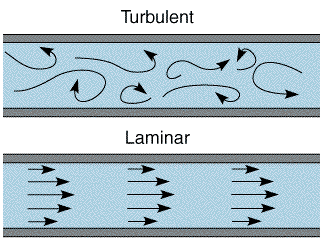
\includegraphics[width=.4\textwidth]{media/laminar_turbulent_orig.png}
\end{center}

\subsubsection{Reynolds number}
Reynolds number is a non-dimensional number that makes the distinction between
laminar and turbolent flows possible. The Reynolds number is given by the
relation between inertial forces and viscous forces:

\figbox{$Re = \dfrac{v\cdot L}{\nu}$}

where:
\begin{itemize}
    \item $v$: velocity $\left[\dfrac{\text{m}}{\text{s}}\right]$;
    \item $L$: characteristic length [m];
    \item $\nu$: kinematic viscosity $\left[\dfrac{\text{m}^2}{\text{s}}\right]$.
\end{itemize}

\subsubsection{Critical Reynolds number}
The transition from laminar to turbolent flow and it's determined by
the critical Reynolds number:
\figbox{
    $Re > 2300 \Rightarrow$ turbulent flow\\
    $Re = 2300 \Rightarrow$ critical point\\
    $Re < 2300 \Rightarrow$ laminar flow
}

\subsubsection{Flow pressure in curvatures}
\begin{center}
    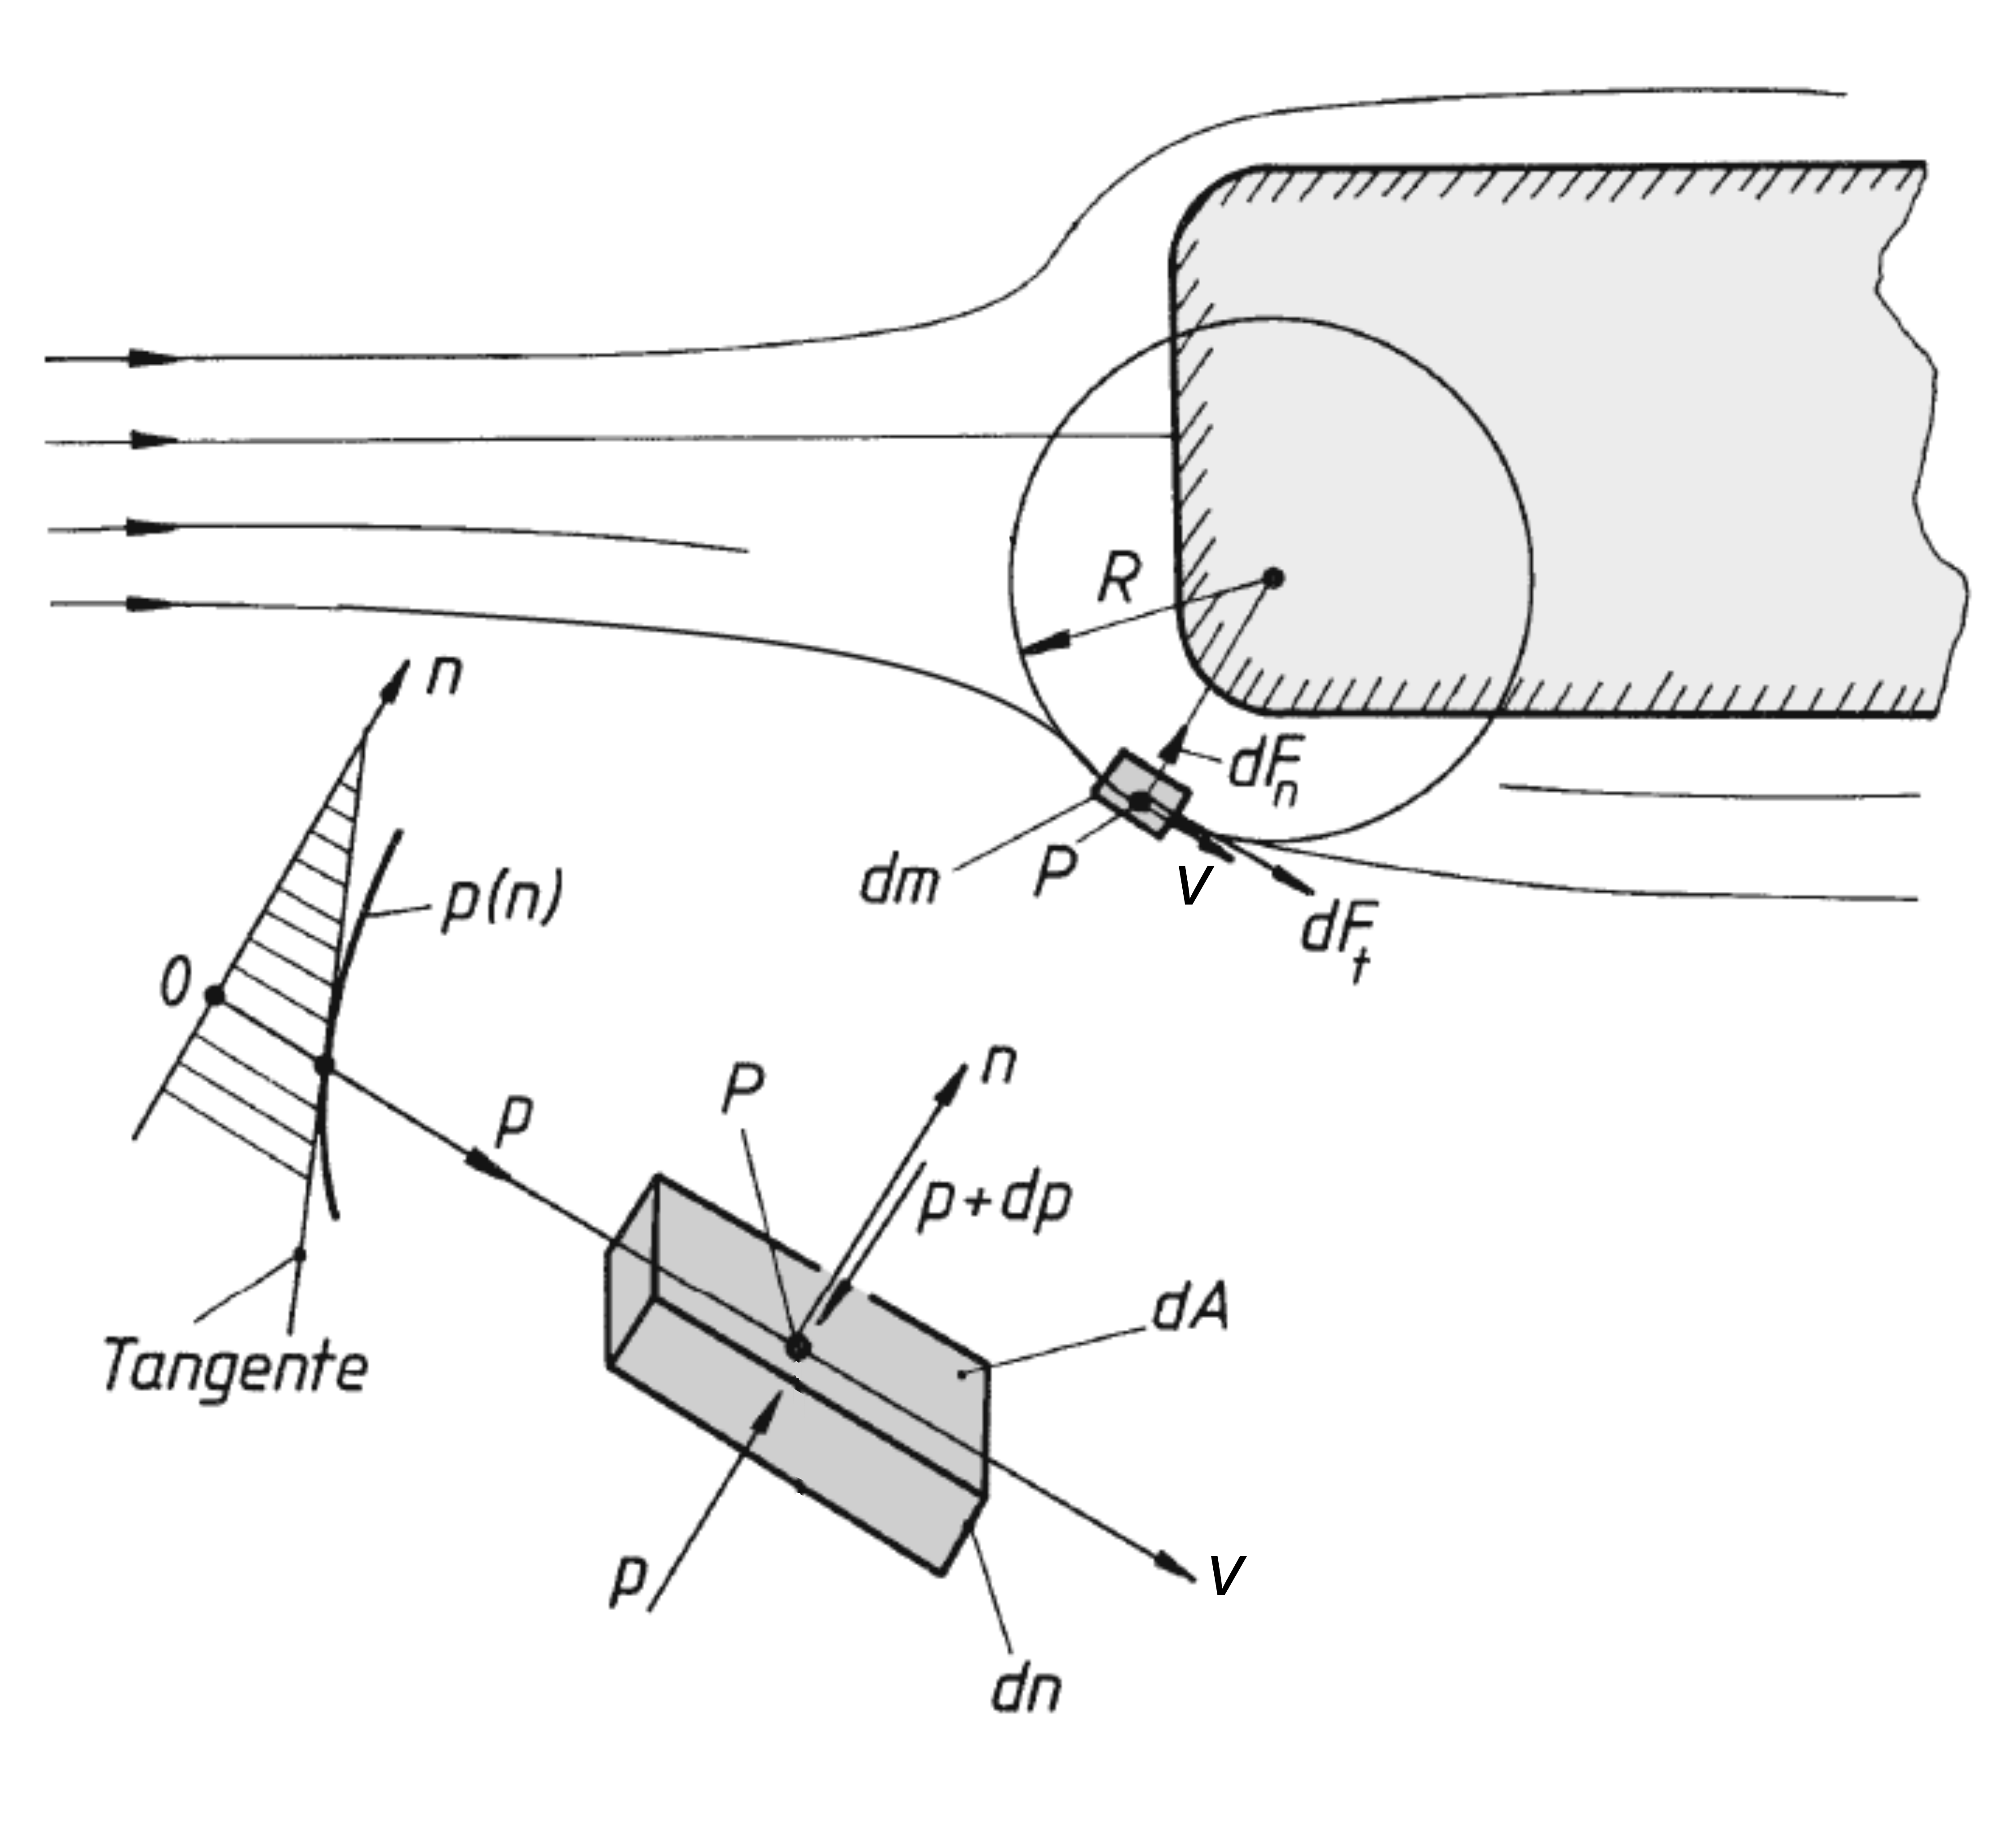
\includegraphics[width=.6\textwidth]{media/Kruemmungsdruck.png}
\end{center}

Force balance of the system:
\[dFn = -dA\left(\left(p+dp\right)-p\right) = dm\cdot a_n\]

where:
\begin{itemize}
    \item $R$: radius of the curvature
    \item $a_n = \dfrac{v^2}{R}$
    \item $dm = g\cdot dA\cdot dn$
\end{itemize}

Pressure in the curvature formulation:
\[\frac{dp}{dn} = -g\cdot \frac{v^2}{R}\]

\subsection{Compressible and incompressible flow}
\subsubsection{Compressible flow}
In compressible flows, the density of the fluid changes so
much that the density change cannot be neglected.

\subsubsection{Incompressible flow}
Fluid flows can be considered incompressible at sufficiently low velocities.
For ideal gases, the speed of sound can be calculated from the state variables and the
fluid properties to:

\figbox{$\dm c=\sqrt{\kappa \cdot R_i \cdot T}$}

If the Mach number is below 0.3, the gas flow can be considered
incompressible.

\figbox{$\dm Ma=\frac{v}{c}=\frac{v}{\sqrt{\kappa \cdot R_i \cdot T}}$}

where:
\begin{itemize}
    \item $v$: fluid velocity $\left[\dfrac{m}{s}\right]$; \\
    \item $c$: speed of sound $\left[\dfrac{m}{s}\right]$; \\
    \item $\kappa$: ssentropic exponent $\left[-\right]$;\\
    \item $R_i$: individual gas constant $\left[\dfrac{J}{kg \cdot K}\right]$;\\
    \item $T$: temperature $\left[K\right]$.
\end{itemize}








\end{document}
